\documentclass[10pt,twocolumn,letterpaper]{article}
\usepackage{cvpr}
\usepackage{graphicx,booktabs,amsmath}
\definecolor{cvprblue}{rgb}{0.21,0.49,0.74}
\usepackage[breaklinks,colorlinks,allcolors=cvprblue]{hyperref}
\def\confName{CVPR}
\def\confYear{2027}
\graphicspath{{figures/}{../results/figures/}}

\title{Few-Shot Industrial Inspection with Aligned Multiscale DINOv2 Patch Matching}
\author{AIAA 3201 Project 2 Team\\Course project report}

\begin{document}
\maketitle
\begin{abstract}
Industrial products often have many normal images and few defect examples. We study whether finer spatial sampling and feature fusion improve normal-only inspection with one to eight reference images. We reproduce AnomalyDINO with frozen DINOv2 at a short edge of 448 pixels and compare it to RGB template difference. Our proposed descriptor aligns final-layer features from 448- and 672-pixel inputs on a common fine grid and retrieves one jointly matched normal patch. Across six VisA categories, fusion improves category-macro image AUROC over AnomalyDINO at 448 by 0.58--1.11 percentage points across four shot counts. With eight references, image AUROC rises from 96.62\% to 97.19\%. At an empirical 4.33\% mean false-positive rate, the point estimate of the miss rate on 195 small-defect images falls from 29.36\% to 25.75\%, with a bootstrap interval for the difference spanning zero. Single-scale 672 gives the best pixel AUROC in the scale-only comparison. Fusion takes longer to run. We examine these trade-offs with matched references, a resolution control and real failures. Code: \url{https://github.com/zero-zhsb/cv_final/tree/codex/final-delivery}.
\end{abstract}

\section{Introduction}
A visual inspection system should flag a defective product and localize the evidence. With only a few verified normal reference images, it must distinguish defects from variations in pose, texture, and illumination without seeing labeled examples of defects.

This problem exposes a difference between detection and localization. An image may be ranked correctly even when the anomaly map responds strongly to unrelated structures. Conversely, a small marked region can receive a local response while the aggregate image score remains below its decision threshold. A high image AUROC is therefore useful evidence about ranking, but it only partly describes the operational consequences of a decision.

We compare three stages of normal-only inspection on the same VisA split~\cite{zou2022visa}. An RGB nearest-template baseline supplies a low-cost comparison. A frozen DINOv2 patch bank implements the AnomalyDINO reference method~\cite{damm2025anomalydino,oquab2024dinov2}. We then test aligned 448+672 fusion against both the unchanged Part 2 at 448 and a single-scale 672 control. The second control is essential because the original AnomalyDINO work already evaluates 672. Our contribution is the controlled comparison of aligned joint retrieval and the corresponding analysis of small defects and compute cost on the course subset.

Our first exploratory experiment combined blocks 6 and 12 at 448. The resulting image ranking improved slightly, but neither block changed the spatial grid. A cashew with two markings occupying about 0.015\% of the original image remained below the rejection threshold. This observation motivated the resolved experiment. We use a finer grid to represent spatial variation and keep a coarse feature at each fine location to test whether the two contextual views help select a normal match.

\paragraph{Contributions.}
We release a matched template baseline, an AnomalyDINO reproduction, and a multiscale descriptor with a fine-resolution control. We evaluate image ranking, pixel localization, small-defect misses, real failures, and GPU cost under a common reference protocol.

\section{Related work}
\paragraph{Normality models and benchmarks.}
MVTec AD~\cite{bergmann2019mvtec} provides images and pixel labels for industrial inspection and helped establish the category-wise unsupervised setting. VisA contains both single-object views and scenes with multiple objects~\cite{zou2022visa}. MVTec AD 2~\cite{heckler2026mvtec2} extends benchmarking to challenging acquisition conditions and image scenarios. We use the six VisA categories defined by the course. Our data do not measure robustness to every acquisition regime.

PaDiM models normal patch embeddings with position-specific distributions~\cite{defard2021padim}. PatchCore uses a representative memory bank and locally aware features~\cite{roth2022patchcore}. Our setting uses exact matching against a bank from very few images. We keep the reference count fixed across comparisons because larger banks can improve coverage of normal appearance without changing the representation.

\paragraph{Synthetic anomalies and prompt learning.}
CutPaste creates pseudo-defects with image transformations for self-supervision~\cite{li2021cutpaste}. DRAEM uses a reconstruction embedding and discriminative training on simulated defects~\cite{zavrtanik2021draem}. Those methods can supply defect-like variation when labels are scarce, but their additional training introduces choices about transfer to real defects. AnomalyCLIP learns object-agnostic text prompts for normality and abnormality~\cite{zhou2024anomalyclip}. We focus on a frozen vision backbone and defer learning a scoring head or a prompt model.

\paragraph{Frozen features and efficient inspection.}
DINOv2 offers transferable patch representations learned without class labels~\cite{oquab2024dinov2}. AnomalyDINO couples them to an exact nearest-normal patch rule, foreground masking and normal reference rotations~\cite{damm2025anomalydino}. General mask models such as Segment Anything~\cite{kirillov2023segment} motivate stronger foreground controls, although foreground suppression cannot resolve every internal reflection or texture mismatch. EfficientAD~\cite{batzner2024efficientad} directly targets low-latency anomaly detection. Its objective motivates reporting latency beside detection quality instead of treating a larger test-time pipeline as a free improvement.

\section{Methods}
\label{sec:methods}

\begin{figure*}[t]
  \centering
  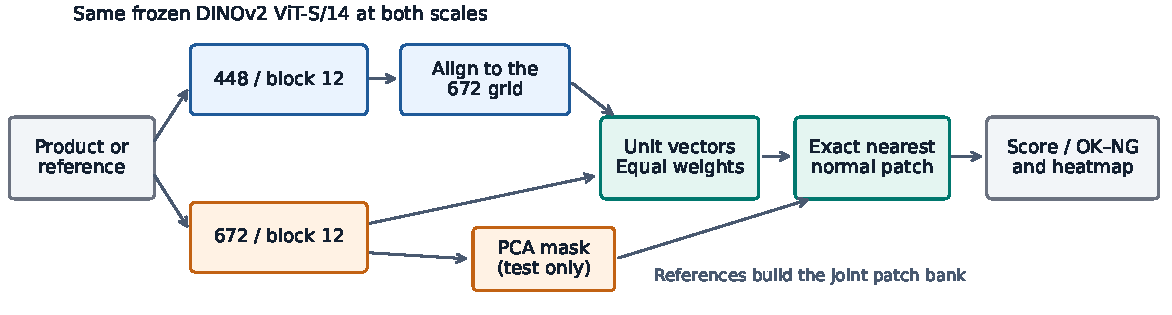
\includegraphics[width=\textwidth]{pipeline.pdf}
  \caption{Aligned multiscale patch matching. The same frozen ViT-S/14 extracts the final block at both sizes. We align coarse features to fine patch centers and retrieve one reference patch using both scales. The two 672-grid methods share the same PCA foreground mask.}
  \label{fig:pipeline}
\end{figure*}

\subsection{Classical nearest-template baseline}
Let \(\mathcal{R}=(R_1,\dots,R_K)\) be normal product images in the manifest. We preserve aspect ratio while resizing the short edge to 448 and crop the right and bottom to multiples of 14. Images are RGB floats in \([0,1]\); no pose registration is fitted. For a test image \(I\) we choose \(j^\ast=\arg\min_j \operatorname{mean}(|I-R_j|)\). We average absolute channel residuals from that template and apply Gaussian smoothing with \(\sigma=1\) at the working resolution. The image score is the mean of the largest 1\% of smoothed residuals. Bilinear resizing returns the map to the size of the original image.

The template baseline uses the same references and tests as the feature methods. Small translations and unfamiliar normal textures can dominate its difference scores.

\subsection{Frozen AnomalyDINO at 448}
The baseline follows the pinned AnomalyDINO data path~\cite{damm2025anomalydino}. The pretrained ViT-S/14 uses a bicubic short-edge resize, patch-aligned crop and ImageNet normalization. We extract the normalized output from block 12. The bank concatenates patch embeddings from the selected normal references and their official rotations, with unit normalization per patch. References use the agnostic path and all reference patches enter the bank. The unchanged PCA foreground rule masks query patches.

For a foreground query descriptor \(z_q\), we compute
\[
 d(q)=\tfrac12\min_{r\in\mathcal B}\|z_q-z_r\|_2^2
\]
by exhaustive floating-point GPU search with TF32 disabled. For a background query we fill the corresponding map with zero. An image is scored by the mean of the largest \(\max(1,\lfloor 0.01 HW\rfloor)\) distances in the full \(H\times W\) patch grid. The original-distance heatmap is reconstructed with bilinear interpolation at original image size and Gaussian smoothing (\(\sigma=4\) original pixels). Rendering does not affect image ranking.

\subsection{Aligned multiscale descriptor}
Figure~\ref{fig:pipeline} summarizes the modified representation. For the same RGB image, we extract the final block at short edges 448 and 672. The short edge then has 32 or 48 tokens. We retain the fine grid as the output grid and sample the coarse descriptor field at each fine patch center using bilinear interpolation. Bilinear sampling provides a coarse contextual descriptor without discarding the fine descriptor at the same location.

Cropping makes this alignment different from stretching one token array to the dimensions of another. Denote the uncropped resized image lengths along an axis by \(a_c\) and \(a_f\). A fine patch at zero-indexed location \(j\) has center \(14(j+\frac12)\) in resized coordinates. Its fractional coordinate on the coarse grid is
\[
 u_c(j)=(j+\tfrac12)\frac{a_c}{a_f}-\tfrac12 .
\]
We apply this independently to both axes and clamp coordinates at the nearest available coarse grid edge. A regression test covers unequal right-edge crops. The local adapter shares the same frozen model between both scales.

For a fine-grid location \(q\), let \(\tilde z_c(q)\) be the sampled coarse embedding and \(z_f(q)\) be the fine embedding. With \(\operatorname{unit}(v)=v/\|v\|_2\), our descriptor is
\[
 z(q)=\frac{1}{\sqrt{2}}
   \left[\operatorname{unit}(\tilde z_c(q));\,
         \operatorname{unit}(z_f(q))\right].
\]
The joint squared distance is the average of the two per-scale squared distances for the \emph{same} normal patch. The chosen patch minimizes the joint distance. Averaging two independently minimized distances would allow two unrelated normal patches to explain one query and changes the tested hypothesis.

We keep official reference rotations, top-1\% aggregation, rendering, and exact search. The single-scale 672 control uses the official 672 feature at each location. Both new methods compute the original PCA mask from the raw block-12 672 descriptors. Identical masks were verified on one normal image per category at eight shots. Using original fine features for the mask separates joint feature retrieval from a change in the background rule.

\subsection{Calibration and decision}
For each category, we reserve the first 20 filename-sorted normal training images. These images never enter a memory bank. After building the bank, we score all 20 using that configuration and set the threshold to the linear 95th percentile. A product is NG when its score exceeds this threshold. Each method uses its own threshold because feature distances and RGB residuals use different scales. All reported AUROCs use continuous scores or pixel values. We explicitly distinguish operating-point analysis from this normal-only demo decision.

\section{Experimental protocol}
\subsection{Data, references, and controls}
We use the official VisA one-class split for candle, capsules, cashew, chewinggum, fryum, and pipe\_fryum. There are 960 distinct test images across the six categories. At \(K\in\{1,2,4,8\}\) and seeds \(s\in\{0,1,2\}\), each category has the same held-out tests. With filename-sorted eligible normal training images, the reference slice is \([sK,(s+1)K)\). The three seed settings correspond to reference slices. They are not three independent test sets. Each method adds 72 category/shot/seed configurations and produces 11,520 prediction rows.

The reference, calibration, test image, label, and mask identities are matched across variants. The original 448 run is retained as the Part 2 reference. The two-scale settings, alignment and weights were fixed before the new test outputs. Earlier test failures motivated the small-defect hypothesis and we treat the new results as controlled comparisons on this benchmark. Independent validation under acquisition changes would be needed for deployment.

The tests include the RGB template, the baseline 448, a 672-only resolution comparison, and 448+672 fusion. The image scales are the intervention, so 448 versus 672 intentionally changes the sampling grid. The 672-only versus fusion comparison holds the final sampling grid, fine-scale mask and reference identities fixed. This allows an estimate of the incremental effect of including coarse contextual features on the fine grid.

\subsection{Metrics and verification}
For each category, shot, and seed we compute image AUROC from the original continuous image scores. Pixel AUROC is computed per category on all original-resolution maps and labels, including all-zero masks for normal products. The maps use the original score scales. We average the six categories equally within each seed and report the mean and population standard deviation over the three seeds. We also show per-category results to expose effects hidden by the overall average.

When large maps overflowed the continuous floating-point key histogram's memory cap, we used exact positive-key ranks. Negative pixels are assigned intervals between the observed positive scores, with exact ties counted separately. This preserves the pairwise AUROC definition and avoids an array spanning every representable score. The implementation was checked against exact AUROC on tied scores and edge cases and verified to run on the original-size 672 maps.

To examine small defects, we fixed a nonempty mask area cutoff of 0.1\% of original pixel count. The resulting subset has 195 distinct abnormal images from all six categories. We report the share of ground-truth pixels falling in the hottest 1\% of an image's map. Ties at the cutoff receive fractional weight so the selected area remains 1\%. This criterion measures concentration at a fixed map budget, while pixel AUROC compares the full ranking.

We also report miss rates at an empirical normal-image false-positive rate capped at 5\%. Within each category and configuration we choose an empirical cutoff from ranked normal test scores for this \emph{evaluation statistic}. The observed mean rate is 4.33\% because the class sample sizes and ties constrain attainable values. The test cutoff is distinct from the normal training threshold used by the demo. The per-category and per-configuration tables accompany the source.

\begin{table*}[t]
\centering
\caption{Mean and population SD of category-macro AUROC in percent. Each cell is image / pixel AUROC. All methods have matched reference and test images. Bold marks the best mean in each metric and shot.}
\label{tab:main}
\setlength{\tabcolsep}{5pt}
\resizebox{\textwidth}{!}{%
\begin{tabular}{lcccc}
\toprule
Method & 1-shot & 2-shot & 4-shot & 8-shot\\
\midrule
RGB template & \(53.17\pm0.53 / 75.98\pm0.63\) & \(56.28\pm3.63 / 76.55\pm0.47\) & \(57.94\pm2.85 / 76.55\pm0.32\) & \(60.80\pm0.32 / 76.91\pm0.33\)\\
AnomalyDINO 448 & \(94.61\pm0.84 / 97.76\pm0.06\) & \(95.33\pm0.46 / 97.92\pm0.07\) & \(96.15\pm0.40 / 98.09\pm0.03\) & \(96.62\pm0.57 / 98.21\pm0.02\)\\
Single-scale 672 & \(94.97\pm0.31 / \mathbf{97.99}\pm0.08\) & \(95.76\pm0.31 / \mathbf{98.14}\pm0.06\) & \(96.29\pm0.20 / \mathbf{98.30}\pm0.05\) & \(96.82\pm0.46 / \mathbf{98.41}\pm0.03\)\\
Fusion 448+672 & \(\mathbf{95.72}\pm0.34 / 97.89\pm0.07\) & \(\mathbf{96.21}\pm0.17 / 98.03\pm0.06\) & \(\mathbf{96.82}\pm0.13 / 98.19\pm0.04\) & \(\mathbf{97.19}\pm0.39 / 98.30\pm0.03\)\\
\bottomrule
\end{tabular}}
\end{table*}

\begin{figure*}[t]
  \centering
  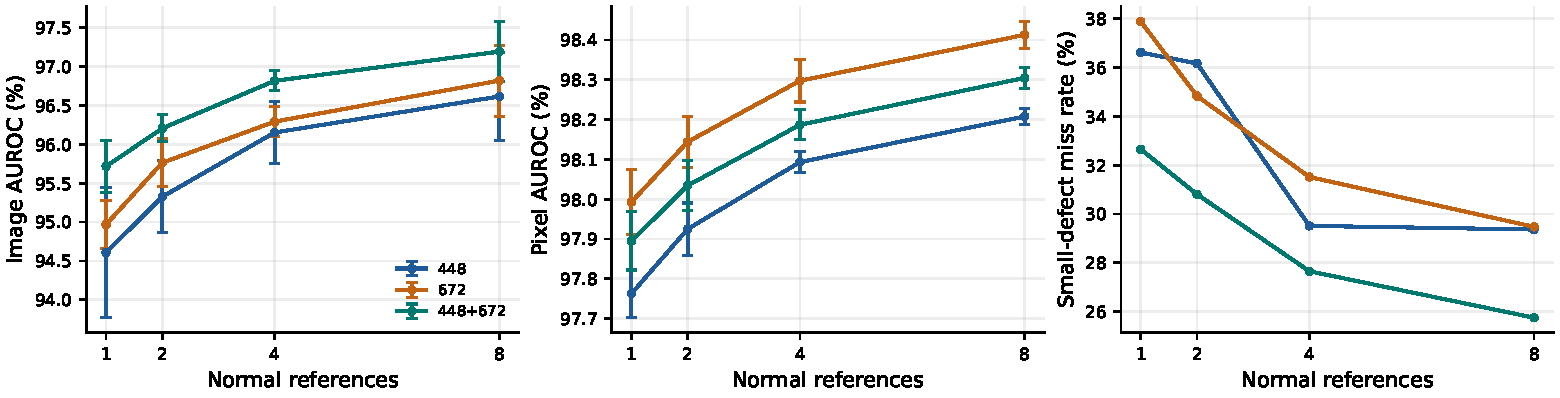
\includegraphics[width=\textwidth]{metrics.pdf}
  \caption{Shot sweeps for the frozen feature methods. AUROC error bars give population SD across the three reference selections. The third plot shows small-defect miss rate at the capped false-positive operating point.}
  \label{fig:metrics}
\end{figure*}

\section{Results and analysis}
\subsection{Overall detection and localization}
Table~\ref{tab:main} gives all four shot counts. The feature methods substantially exceed RGB template difference. At 8-shot the template attains 60.80\% image and 76.91\% pixel AUROC. The 448 model attains 96.62\% and 98.21\%, consistent with richer normal patch representations providing a more transferable comparison than matched raw RGB.

The 672 control increases pixel AUROC by 0.20--0.23 percentage points across the four shot counts. It also improves mean image AUROC over 448, with increases between 0.14 and 0.44 points. This supports the hypothesis that more finely sampled patches represent relevant spatial differences in this data. A change in resolution also changes the spatial footprint and the foreground mask, so the 448 versus 672 comparison is a bundled resolution effect.

Fusion raises image AUROC above 672 by 0.37--0.75 points across shot settings. This gain is present in all 12 shot--seed comparisons after category averaging. For example the 8-shot gains over 672 are 0.44, 0.27, and 0.41 points. At 1-shot the gain over 448 is 1.11 points on average. Three reference selections with a shared test set cannot establish generalization to independent products, and these paired directions should be read accordingly.

We additionally use 4,000 image bootstrap replicates stratified by category and label. A resampled image is paired across methods and reference selections. At 1-shot, the gain over 448 is 1.11 points (95\% percentile interval [0.50, 1.74]) and the gain over 672 is 0.75 [0.30, 1.20]. Both intervals stay above zero after a Bonferroni adjustment across four shots and two controls. At 8-shot, the gain over 448 is 0.58 [0.10, 1.07] points, with an adjusted interval of [$-0.07$, 1.25]. The clearest evidence is therefore in the one-reference setting. These intervals quantify test-image resampling variability conditional on the six categories and the chosen reference sets.

The same fusion loses 0.10--0.11 points of pixel AUROC relative to 672. The coarse contextual term can change the match that minimizes the joint distance, including matches for normal pixels. The divergence between image and pixel AUROC is consistent with improvement in the largest image-level responses even when many other pixels become slightly less well ranked. It makes the strong 672-only control important for selecting a method according to the final use.

\begin{table}[t]
\centering
\caption{Image / pixel AUROC (\%) by category at 8-shot, averaged over seeds.}
\label{tab:category}
\setlength{\tabcolsep}{3pt}
\begin{tabular}{lccc}
\toprule
Category & 448 & 672 & 448+672\\
\midrule
Candle & 93.47 / 98.38 & 94.31 / 99.20 & 94.60 / 99.15\\
Capsules & 98.13 / 95.59 & 98.90 / 95.40 & 98.98 / 95.24\\
Cashew & 94.62 / 99.32 & 95.62 / 99.49 & 95.85 / 99.51\\
Chewinggum & 98.87 / 99.55 & 98.75 / 99.47 & 98.86 / 99.49\\
Fryum & 98.11 / 97.21 & 97.59 / 97.64 & 98.45 / 97.18\\
Pipe fryum & 96.49 / 99.19 & 95.75 / 99.28 & 96.41 / 99.28\\
\bottomrule
\end{tabular}
\end{table}

\subsection{Where the gains come from}
Table~\ref{tab:category} shows why the aggregate comparison is not a uniform improvement. In the eight-reference setting, the image AUROC gain over 448 is about 1.23 points for cashew and 1.13 for candle. Chewinggum and pipe fryum are slightly lower. Capsules improve in image ranking while their pixel AUROC falls as features become more detailed. Fryum illustrates the scale contribution clearly: fusion recovers the image ranking lost by switching from 448 to 672 and slightly exceeds 448, while the 672 grid alone has the highest pixel ranking.

At fixed resolution, our earlier layer study helps interpret this result. The sixth block alone ranks images worse than the twelfth block at every shot setting. Equal layer fusion at 448 improves image AUROC over block 12 by only 0.19--0.28 points. Since that combination does not change the grid, it provides little evidence for better localization of the smallest regions. We present the resolution experiment as the main improvement and treat the layer experiment as an exploratory ablation.

\subsection{Small-defect operating point}
At eight references, the share of tiny-defect GT pixels in the hottest 1\% rises from 88.78\% for 448 to 92.26\% for 672 and 92.50\% with fusion. The largest gain comes from finer sampling. At the same observed 4.33\% mean normal false-positive rate, 672 has a small-defect miss rate of 29.47\% and fusion has 25.75\%. The unchanged 448 rate is 29.36\%. Thus the finer control better concentrates hotspot pixels while joint features improve which images cross the low-false-alarm operating point. Figure~\ref{fig:metrics} gives the same breakdown over shot counts. The analysis does not establish the miss rate of a threshold calibrated on another line.

To quantify uncertainty at this operating point, we use 4,000 paired bootstrap draws of normal and tiny-defect images within each category. We estimate the capped FPR threshold again in every draw. Identical draws pair the methods and the three reference selections. At 8-shot the fusion-minus-448 estimate is $-3.62$ points, with a 95\% percentile interval [$-10.45$, $+2.06$]. Relative to 672 the estimate is $-3.72$ [$-7.86$, $+1.23$] points. The intervals include zero, so the lower observed miss rate should be treated as a trend on this subset.

\begin{figure*}[t]
  \centering
  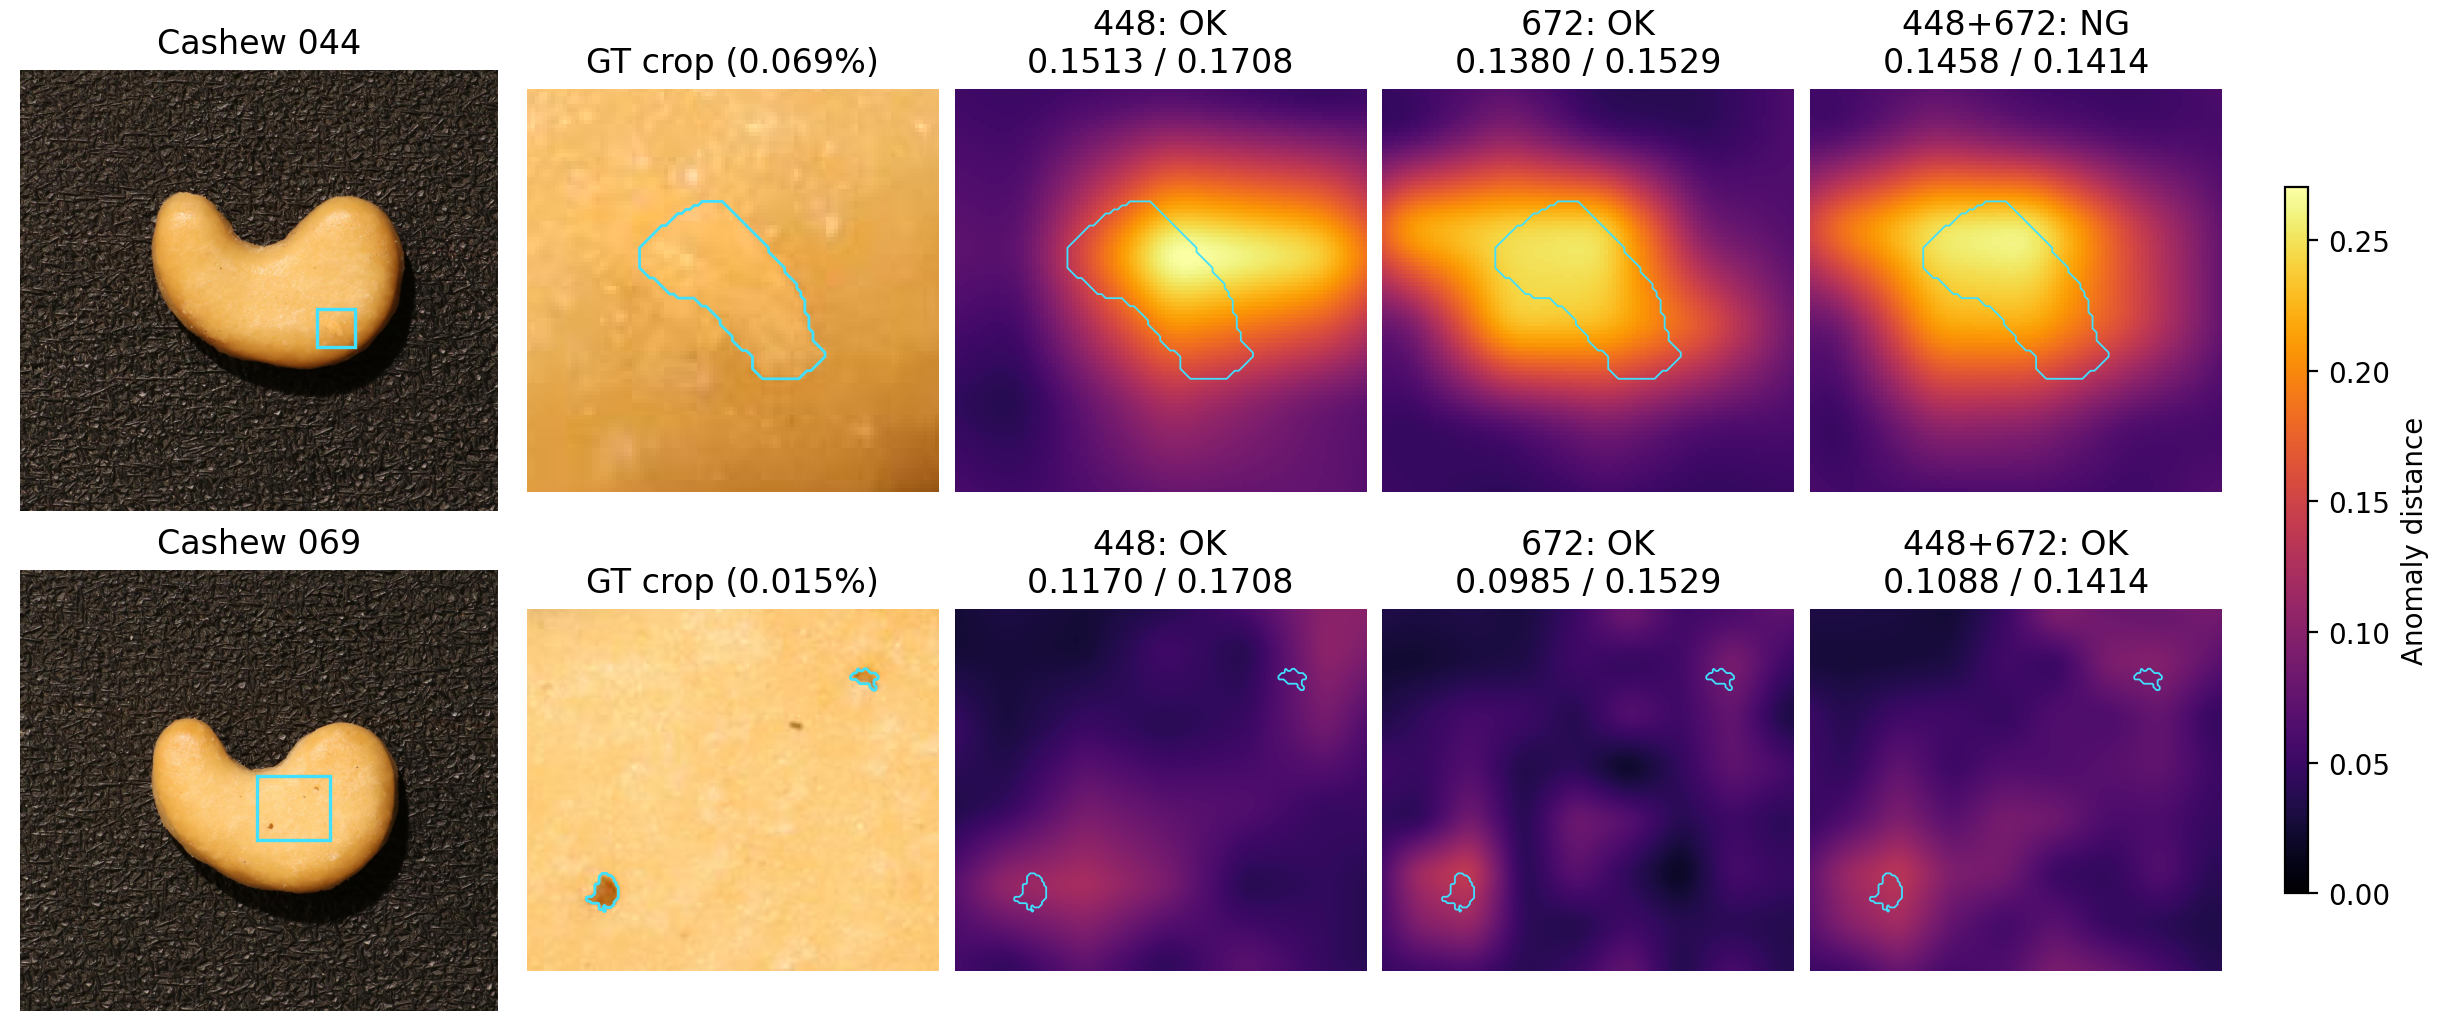
\includegraphics[width=\textwidth]{cashew_pair.png}
  \caption{Matched detail crops from genuine single-image inference at 8-shot, seed 0. The turquoise outline marks the evaluation mask. All maps use the same raw color scale. Cashew 044 is detected by the fused method, whereas cashew 069 remains below all three normal-only calibrated thresholds. The mask is used only to display the crop after scoring.}
  \label{fig:cashew}
\end{figure*}

\subsection{Matched success and persistent failure}
Figure~\ref{fig:cashew} compares two very small defects on the same product class. The masks cover approximately 0.0695\% and 0.0147\% of full-image pixels. For 044, 448 scores 0.1513 against a threshold of 0.1708 and 672 scores 0.1380 against 0.1529. Fusion reaches 0.1458 against 0.1414. These separate operating thresholds follow the same per-category normal-only quantile rule. The picture illustrates a change in a real decision and is not a statistic of improvement on its own.

The second image, 069, remains an OK output even with fine sampling. Its largest distances remain insufficient to clear the score aggregation threshold. On both images, local responses can be visible while a small mark contributes little to the top-percentile mean over the entire grid. The contrast between the two cases motivates reporting image scores, cropped heatmaps, and image-level labels together.

\subsection{Five difficult cases}
Figure~\ref{fig:failures} shows five genuine errors at 8-shot seed 0, prioritizing different categories and large relative threshold errors. These images serve as failure diagnostics. Three have normal labels and are rejected by all three feature methods. The pipe fryum response follows an internal stripe. The chewinggum hotspot lies near a bright edge, consistent with a reflection. The candle response concentrates on the lower right rim. These normal patches share the product region with actual defects, which explains why masking only background patches cannot directly suppress their responses.

The remaining two images are defective yet all three feature methods accept them. In capsules 066 the representation responds across several capsules, and the marked upper-left capsule does not stand out strongly enough at the image level. In cashew 071 the ground truth is small and sparse. A fine anomaly map can show a weak feature near the marks without producing a sufficiently high aggregate. We do not assign a physical failure cause where the image only supports a visual association.

\begin{figure*}[t]
  \centering
  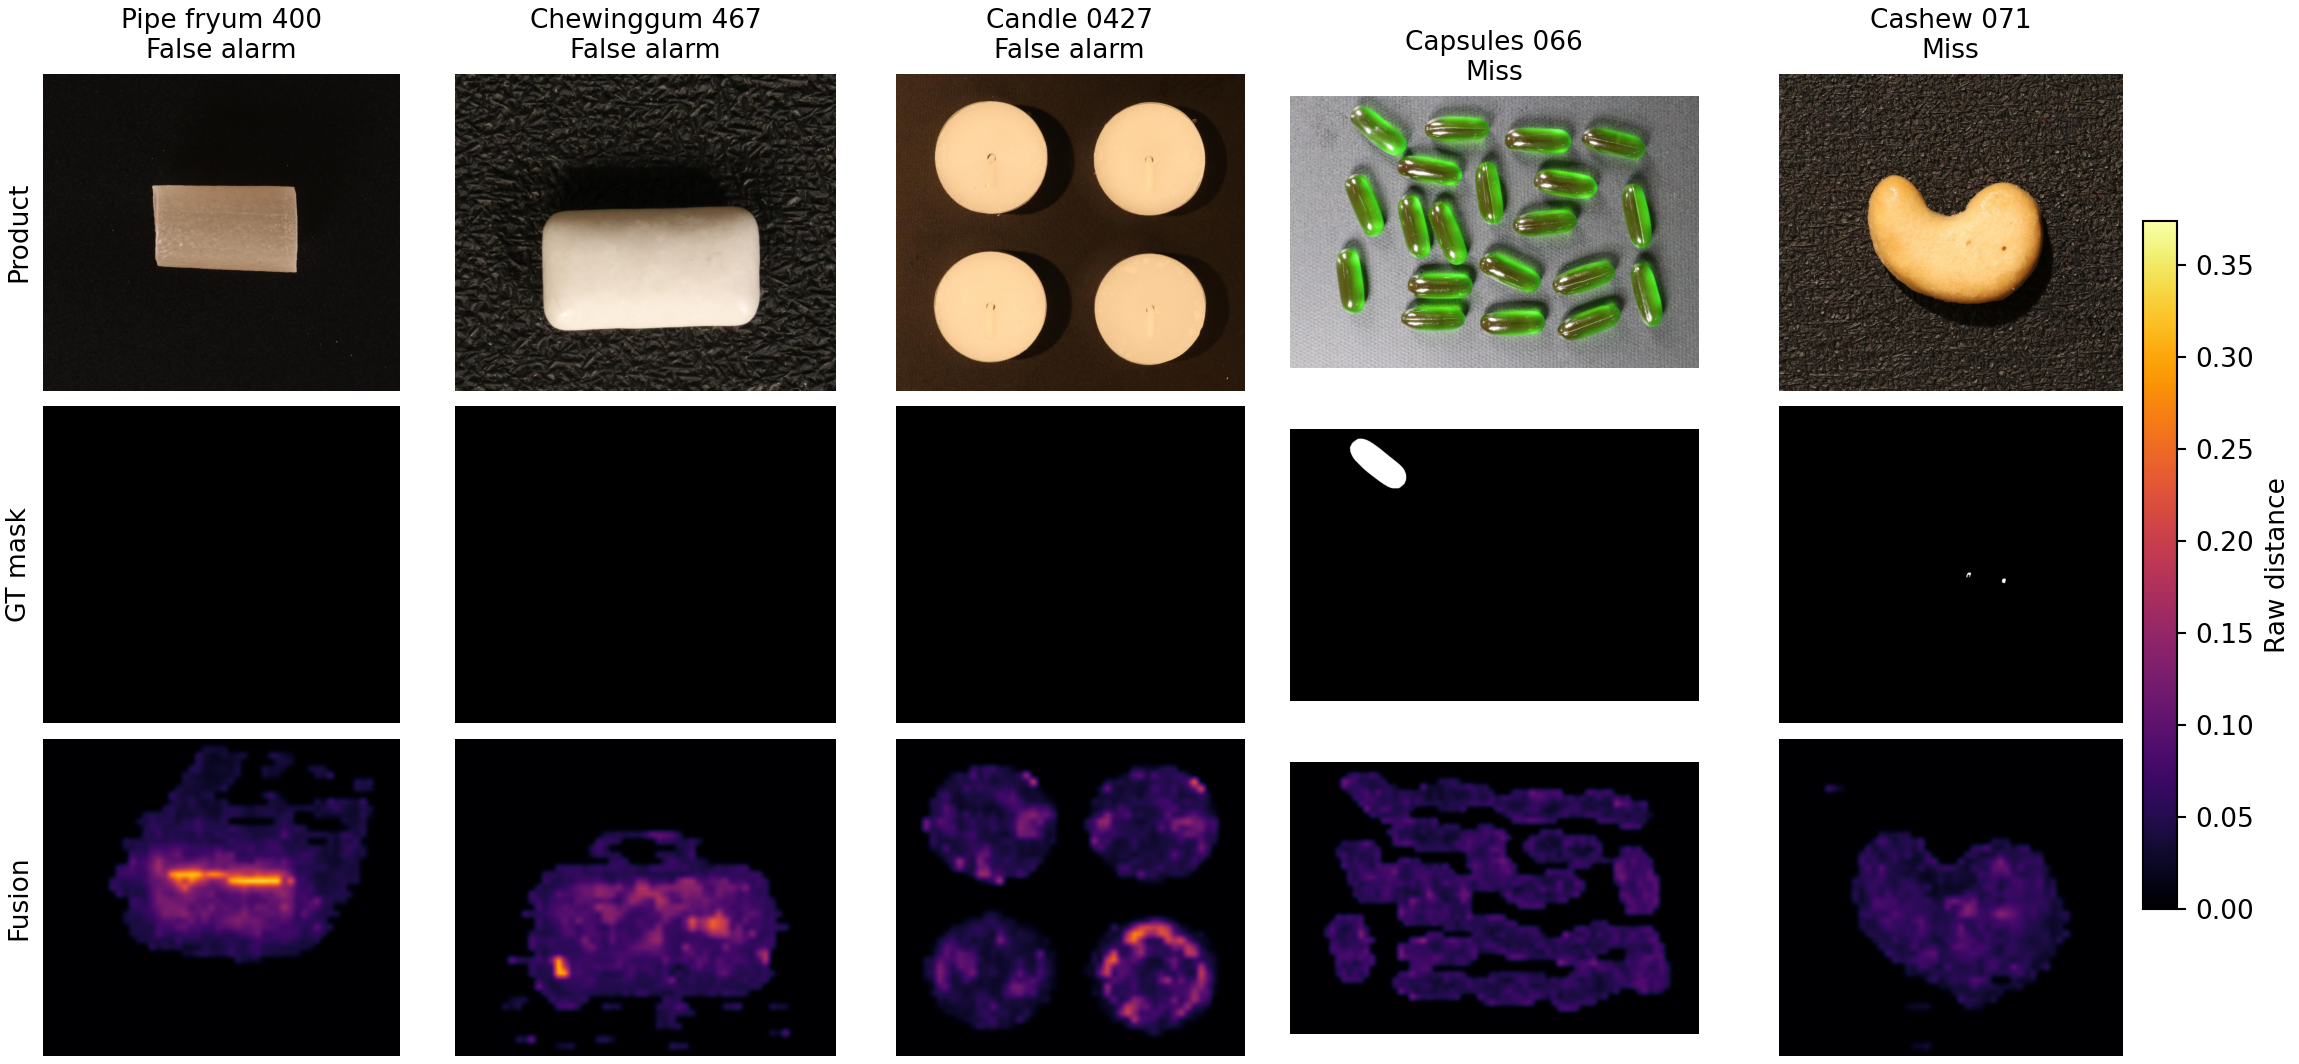
\includegraphics[width=.96\textwidth]{failure_gallery.png}
  \caption{Five selected difficult images. The rows show the original product, its ground-truth mask, and the fused method's map on a shared raw scale. The first three columns are false alarms and the last two are missed defects. The repository contains full-size maps from the two controls and the calibrated scores for all five images.}
  \label{fig:failures}
\end{figure*}

\section{Efficiency and demonstration}
\begin{table}[t]
\centering
\caption{Same-session RTX A6000 results. Time is the mean per image and memory is the largest peak PyTorch allocation across the sampled configurations.}
\label{tab:efficiency}
\begin{tabular}{lrrr}
\toprule
Method & Shot & ms/image & Peak MiB\\
\midrule
448 & 1 & 72.14 & 149.55\\
672 & 1 & 117.69 & 233.51\\
448+672 & 1 & 171.09 & 277.29\\
448 & 8 & 73.30 & 381.58\\
672 & 8 & 142.07 & 742.05\\
448+672 & 8 & 205.81 & 1390.05\\
\bottomrule
\end{tabular}
\end{table}

Table~\ref{tab:efficiency} compares variants on one shared RTX A6000. We alternate the order cyclically across category and shot blocks. Each method uses identical inputs within a block, two normal and two abnormal, repeated three times after warm-up. Time includes reading the image, input transforms, feature extraction, masking, and exact patch search. Reference construction, heatmap interpolation, file export, and evaluation are measured separately or outside the timed span.

The relative costs reflect an additional model pass and a larger feature bank. At eight shots the fine-grid bank contains more tokens than the 448 bank and fusion doubles the descriptor dimension at that grid. Single-scale 672 offers stronger aggregate localization and lower computational cost. Fusion makes a case when image ranking and misses at a specified operating point dominate the decision. The benchmark order reduces load effects but does not isolate the shared device, and the reported numbers should not be extrapolated to production throughput.

A product-image CLI provides the normal-only inspection demonstration. It builds the reference bank from the explicit manifest, derives the 95th-percentile threshold from the reserved normal images and runs fresh inference on the provided product image. It exports the image score, threshold, OK/NG, original-size heatmap and overlay. We verified four methods on one normal case, one tiny defect recovered by fusion, and another persistent miss. No ground-truth mask is read by the CLI. Evaluation figures add only the official VisA mask after prediction.

\subsection{Exploratory comparison with an OAS metric}
Oracle approximating shrinkage (OAS)~\cite{chen2010oas} fits a covariance on reference descriptors. We whiten all 768 dimensions and scale by $1/\sqrt{768}$ before matching. The 20 calibration images fit only the threshold. At 8-shot, pixel AUROC rises from 98.30\% to 98.63\%, while image AUROC drops from 97.19\% to 97.08\%. At 1-shot the pixel gain is 0.52 points and the image loss is 1.21. We selected this distance rule after exploratory work on the same benchmark. The main scale study and the paired efficiency comparison use the original metric.

\section{Conclusion and limitations}
The strongest system depends on the target metric. Aligned spatial fusion consistently improves image AUROC over the two single-scale controls on the six category averages. We observe fewer small-defect misses at the matched low-false-alarm operating point, with substantial uncertainty on that subset. A single high-resolution view yields the best overall pixel AUROC among the three scale variants and greater efficiency than fusion. An exploratory OAS metric improves pixel ranking further at a cost to image ranking. Matching information from two contextual scales helps image decisions in this study, while the fine grid and distance rule affect pixel localization.

The experiments are confined to one public benchmark, six categories, and three reference selections per shot. They provide no estimate of cross-camera or production-line robustness. The previous test analysis informed our hypothesis, and the fixed-scale comparison should be interpreted in that context. The empirical FPR cap provides a comparative benchmark, whereas the limited normal calibration pool gives a threshold whose realized false-positive rate can differ on a new line. Future work should profile feature extraction and search individually and evaluate whether avoiding the coarse pass on easy images preserves small-defect recall. An independent validation set would be needed to choose a routing rule before testing it.

\paragraph{Reproducibility and attribution.}
The repository provides the manifest, version and weight pins, per-configuration metrics, and demo outputs. VisA images and masks are by Zou et al.~\cite{zou2022visa}, CC BY 4.0. Our preprocessing and scoring follow AnomalyDINO~\cite{damm2025anomalydino}, with frozen DINOv2 weights~\cite{oquab2024dinov2}.

{\small
\bibliographystyle{ieeenat_fullname}
\bibliography{references}
}
\end{document}
